\documentclass[../../main.tex]{subfiles}

\begin{document}

\section{Motivation}

Machine learning models have been immensely successful in variety of applications to generate predictions in data-driven driven domains such as computer vision, robotics, weather forecasting. While the success of these models is undeniable, we lack the ability to understand the uncertaincy in the predictions made by most of the State-of-the-Art models. This is a major drawback in the deployment of these models in real-world applications, for example, in weather forecasting, it is important to know the uncertaincy in the prediction of the weather as this information is arguably as valuable as the prediction itself. In this work, we aim to implement a model is \textbf{Uncertainty-Aware} whilst also posessing further desirable properties.

\section{Desirable Properties}

Ontop of being uncertaincy aware, we would like to insert some desirable inductive biases that help the model to generalize better and be more interpretable. We would like the model to be able to:

\textbf{Permutation Invariant}: \emph{The prediction of the model should not change if the order of the input data is changed}. When each datapoint contains the information about input and output pairs, the model should not care about the order in which they are fed into the model. For example, in the case of a weather forecasting model using data from multiple weather stations, the model should not care about the order in which the data from the weather stations is fed into the model, thus making the model permutation invariant.

\textbf{Translation Equivariant}: \emph{Shifting the input data by a constant amount should result in a constant shift in the predictions}. For example, in the case of a weather forecasting model, if the data from the weather stations is shifted by a constant amount, the model should be able to predict the same shift in the weather forecast.

\begin{figure}[H]
	\centering
	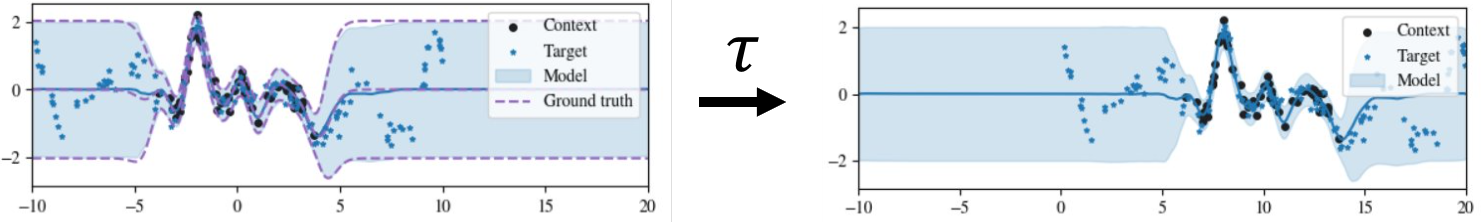
\includegraphics[width=0.9\textwidth]{./te.PNG}
	\caption{The Translation Equivariant property. Consider the given prediction on the black datapoints on the left. If the input is shifted by a constant amount, the prediction should also shift by the same amount (right).}
	\label{fig:te}
\end{figure}


\todo{Clearer figure}

\autoref{fig:te} illustrates the Translation Equivariant (TE) property on a simple 1D dataset. If the model, $f$ is TE then the following holds:

\begin{align}
	&f: \bm{x} \rightarrow (\bm{x}, \bm{\hat{y}}) \\
	&f: \bm{x} + \bm{c} \rightarrow (\bm{x} + \bm{c}, \bm{\hat{y}})
\end{align}

Where $\bm{x}$ is the input and $\bm{\hat{y}}$ is the output and $\bm{c}$ is a constant shift in the input.


\textbf{Off-the-Grid Generalization}: \emph{The model should be able to work on off-the-grid data points}. Off-the-grid data points are the data points that are not in a regular gridded structure, for example, images that are missing pixel values are off-the-grid. Traditional models like Convolutional Neural Networks (CNNs) are not able to work on off-the-grid data points since they require a regular structure to apply the convolution operation. By making the model off-the-grid generalizable, we can create models that can work on many different types of data and easily handle missing data points. It also allows the model to generalize to regions of the input space that it has not seen during training. Tasks like image inpainting, where the model is required to fill in missing pixels in an image, can benefit from this property.

\todo{Add a figure to illustrate off-the-grid generalization}





\ifSubfilesClassLoaded{%
    \printbibliography{}
}{} 


\end{document}